\documentclass[letterpaper]{IEEEtran}
%
% If IEEEtran.cls has not been installed into the LaTeX system files,
% manually specify the path to it like:
% \documentclass[journal]{../sty/IEEEtran}

% LAURO
\usepackage{listings}
\usepackage[table]{xcolor}
% ---
% cores
% ---
\definecolor{dkgreen}{rgb}{0,0.6,0}
\definecolor{gray}{rgb}{0.5,0.5,0.5}
\definecolor{mauve}{rgb}{0.58,0,0.82}

\lstset{frame=tb,
  language=Python,
  aboveskip=3mm,
  belowskip=3mm,
  showstringspaces=false,
  columns=flexible,
  basicstyle={\small\ttfamily},
  numbers=none,
  numberstyle=\tiny\color{gray},
  keywordstyle=\color{blue},
  commentstyle=\color{dkgreen},
  stringstyle=\color{mauve},
  breaklines=true,
  breakatwhitespace=true,
  tabsize=4
}
% END LAURO




% Some very useful LaTeX packages include:
% (uncomment the ones you want to load)


% *** MISC UTILITY PACKAGES ***
\usepackage{graphicx}
\graphicspath{{images/}}
\usepackage{capt-of}
\usepackage{amsmath}
%\usepackage[spanish]{babel}
%\usepackage[utf8]{inputenc}
%\usepackage[latin1]{inputenc}
\usepackage{rotating}
\usepackage{subfig}
\usepackage{hyphenat}
%\usepackage[papersize={216mm,330mm},tmargin=15mm,bmargin=15mm,lmargin=15mm,rmargin=15mm]{geometry}


% (utf8x si hay problemas)
%
%\usepackage{ifpdf}
% Heiko Oberdiek's ifpdf.sty is very useful if you need conditional
% compilation based on whether the output is pdf or dvi.
% usage:
% \ifpdf
%   % pdf code
% \else
%   % dvi code
% \fi
% The latest version of ifpdf.sty can be obtained from:
% http://www.ctan.org/tex-archive/macros/latex/contrib/oberdiek/
% Also, note that IEEEtran.cls V1.7 and later provides a builtin
% \ifCLASSINFOpdf conditional that works the same way.
% When switching from latex to pdflatex and vice-versa, the compiler may
% have to be run twice to clear warning/error messages.






% *** CITATION PACKAGES ***
%
\usepackage{cite}
% cite.sty was written by Donald Arseneau
% V1.6 and later of IEEEtran pre-defines the format of the cite.sty package
% \cite{} output to follow that of IEEE. Loading the cite package will
% result in citation numbers being automatically sorted and properly
% "compressed/ranged". e.g., [1], [9], [2], [7], [5], [6] without using
% cite.sty will become [1], [2], [5]--[7], [9] using cite.sty. cite.sty's
% \cite will automatically add leading space, if needed. Use cite.sty's
% noadjust option (cite.sty V3.8 and later) if you want to turn this off
% such as if a citation ever needs to be enclosed in parenthesis.
% cite.sty is already installed on most LaTeX systems. Be sure and use
% version 5.0 (2009-03-20) and later if using hyperref.sty.
% The latest version can be obtained at:
% http://www.ctan.org/tex-archive/macros/latex/contrib/cite/
% The documentation is contained in the cite.sty file itself.






% *** GRAPHICS RELATED PACKAGES ***
%
\ifCLASSINFOpdf
  % \usepackage[pdftex]{graphicx}
  % declare the path(s) where your graphic files are
  % \graphicspath{{../pdf/}{../jpeg/}}
  % and their extensions so you won't have to specify these with
  % every instance of \includegraphics
  % \DeclareGraphicsExtensions{.pdf,.jpeg,.png}
\else
  % or other class option (dvipsone, dvipdf, if not using dvips). graphicx
  % will default to the driver specified in the system graphics.cfg if no
  % driver is specified.
  % \usepackage[dvips]{graphicx}
  % declare the path(s) where your graphic files are
  % \graphicspath{{../eps/}}
  % and their extensions so you won't have to specify these with
  % every instance of \includegraphics
  % \DeclareGraphicsExtensions{.eps}
\fi
% graphicx was written by David Carlisle and Sebastian Rahtz. It is
% required if you want graphics, photos, etc. graphicx.sty is already
% installed on most LaTeX systems. The latest version and documentation
% can be obtained at:
% http://www.ctan.org/tex-archive/macros/latex/required/graphics/
% Another good source of documentation is "Using Imported Graphics in
% LaTeX2e" by Keith Reckdahl which can be found at:
% http://www.ctan.org/tex-archive/info/epslatex/
%
% latex, and pdflatex in dvi mode, support graphics in encapsulated
% postscript (.eps) format. pdflatex in pdf mode supports graphics
% in .pdf, .jpeg, .png and .mps (metapost) formats. Users should ensure
% that all non-photo figures use a vector format (.eps, .pdf, .mps) and
% not a bitmapped formats (.jpeg, .png). IEEE frowns on bitmapped formats
% which can result in "jaggedy"/blurry rendering of lines and letters as
% well as large increases in file sizes.
%
% You can find documentation about the pdfTeX application at:
% http://www.tug.org/applications/pdftex





% *** MATH PACKAGES ***
%
%\usepackage[cmex10]{amsmath}
% A popular package from the American Mathematical Society that provides
% many useful and powerful commands for dealing with mathematics. If using
% it, be sure to load this package with the cmex10 option to ensure that
% only type 1 fonts will utilized at all point sizes. Without this option,
% it is possible that some math symbols, particularly those within
% footnotes, will be rendered in bitmap form which will result in a
% document that can not be IEEE Xplore compliant!
%
% Also, note that the amsmath package sets \interdisplaylinepenalty to 10000
% thus preventing page breaks from occurring within multiline equations. Use:
%\interdisplaylinepenalty=2500
% after loading amsmath to restore such page breaks as IEEEtran.cls normally
% does. amsmath.sty is already installed on most LaTeX systems. The latest
% version and documentation can be obtained at:
% http://www.ctan.org/tex-archive/macros/latex/required/amslatex/math/





% *** SPECIALIZED LIST PACKAGES ***
%
%\usepackage{algorithmic}
% algorithmic.sty was written by Peter Williams and Rogerio Brito.
% This package provides an algorithmic environment fo describing algorithms.
% You can use the algorithmic environment in-text or within a figure
% environment to provide for a floating algorithm. Do NOT use the algorithm
% floating environment provided by algorithm.sty (by the same authors) or
% algorithm2e.sty (by Christophe Fiorio) as IEEE does not use dedicated
% algorithm float types and packages that provide these will not provide
% correct IEEE style captions. The latest version and documentation of
% algorithmic.sty can be obtained at:
% http://www.ctan.org/tex-archive/macros/latex/contrib/algorithms/
% There is also a support site at:
% http://algorithms.berlios.de/index.html
% Also of interest may be the (relatively newer and more customizable)
% algorithmicx.sty package by Szasz Janos:
% http://www.ctan.org/tex-archive/macros/latex/contrib/algorithmicx/




% *** ALIGNMENT PACKAGES ***
%
%\usepackage{array}
% Frank Mittelbach's and David Carlisle's array.sty patches and improves
% the standard LaTeX2e array and tabular environments to provide better
% appearance and additional user controls. As the default LaTeX2e table
% generation code is lacking to the point of almost being broken with
% respect to the quality of the end results, all users are strongly
% advised to use an enhanced (at the very least that provided by array.sty)
% set of table tools. array.sty is already installed on most systems. The
% latest version and documentation can be obtained at:
% http://www.ctan.org/tex-archive/macros/latex/required/tools/


% IEEEtran contains the IEEEeqnarray family of commands that can be used to
% generate multiline equations as well as matrices, tables, etc., of high
% quality.




% *** SUBFIGURE PACKAGES ***
%\ifCLASSOPTIONcompsoc
%  \usepackage[caption=false,font=normalsize,labelfont=sf,textfont=sf]{subfig}
%\else
%  \usepackage[caption=false,font=footnotesize]{subfig}
%\fi
% subfig.sty, written by Steven Douglas Cochran, is the modern replacement
% for subfigure.sty, the latter of which is no longer maintained and is
% incompatible with some LaTeX packages including fixltx2e. However,
% subfig.sty requires and automatically loads Axel Sommerfeldt's caption.sty
% which will override IEEEtran.cls' handling of captions and this will result
% in non-IEEE style figure/table captions. To prevent this problem, be sure
% and invoke subfig.sty's "caption=false" package option (available since
% subfig.sty version 1.3, 2005/06/28) as this is will preserve IEEEtran.cls
% handling of captions.
% Note that the Computer Society format requires a larger sans serif font
% than the serif footnote size font used in traditional IEEE formatting
% and thus the need to invoke different subfig.sty package options depending
% on whether compsoc mode has been enabled.
%
% The latest version and documentation of subfig.sty can be obtained at:
% http://www.ctan.org/tex-archive/macros/latex/contrib/subfig/




% *** FLOAT PACKAGES ***
%
%\usepackage{fixltx2e}
% fixltx2e, the successor to the earlier fix2col.sty, was written by
% Frank Mittelbach and David Carlisle. This package corrects a few problems
% in the LaTeX2e kernel, the most notable of which is that in current
% LaTeX2e releases, the ordering of single and double column floats is not
% guaranteed to be preserved. Thus, an unpatched LaTeX2e can allow a
% single column figure to be placed prior to an earlier double column
% figure. The latest version and documentation can be found at:
% http://www.ctan.org/tex-archive/macros/latex/base/


%\usepackage{stfloats}
% stfloats.sty was written by Sigitas Tolusis. This package gives LaTeX2e
% the ability to do double column floats at the bottom of the page as well
% as the top. (e.g., "\begin{figure*}[!b]" is not normally possible in
% LaTeX2e). It also provides a command:
%\fnbelowfloat
% to enable the placement of footnotes below bottom floats (the standard
% LaTeX2e kernel puts them above bottom floats). This is an invasive package
% which rewrites many portions of the LaTeX2e float routines. It may not work
% with other packages that modify the LaTeX2e float routines. The latest
% version and documentation can be obtained at:
% http://www.ctan.org/tex-archive/macros/latex/contrib/sttools/
% Do not use the stfloats baselinefloat ability as IEEE does not allow
% \baselineskip to stretch. Authors submitting work to the IEEE should note
% that IEEE rarely uses double column equations and that authors should try
% to avoid such use. Do not be tempted to use the cuted.sty or midfloat.sty
% packages (also by Sigitas Tolusis) as IEEE does not format its papers in
% such ways.
% Do not attempt to use stfloats with fixltx2e as they are incompatible.
% Instead, use Morten Hogholm'a dblfloatfix which combines the features
% of both fixltx2e and stfloats:
%
% \usepackage{dblfloatfix}
% The latest version can be found at:
% http://www.ctan.org/tex-archive/macros/latex/contrib/dblfloatfix/




%\ifCLASSOPTIONcaptionsoff
%  \usepackage[nomarkers]{endfloat}
% \let\MYoriglatexcaption\caption
% \renewcommand{\caption}[2][\relax]{\MYoriglatexcaption[#2]{#2}}
%\fi
% endfloat.sty was written by James Darrell McCauley, Jeff Goldberg and
% Axel Sommerfeldt. This package may be useful when used in conjunction with
% IEEEtran.cls'  captionsoff option. Some IEEE journals/societies require that
% submissions have lists of figures/tables at the end of the paper and that
% figures/tables without any captions are placed on a page by themselves at
% the end of the document. If needed, the draftcls IEEEtran class option or
% \CLASSINPUTbaselinestretch interface can be used to increase the line
% spacing as well. Be sure and use the nomarkers option of endfloat to
% prevent endfloat from "marking" where the figures would have been placed
% in the text. The two hack lines of code above are a slight modification of
% that suggested by in the endfloat docs (section 8.4.1) to ensure that
% the full captions always appear in the list of figures/tables - even if
% the user used the short optional argument of \caption[]{}.
% IEEE papers do not typically make use of \caption[]'s optional argument,
% so this should not be an issue. A similar trick can be used to disable
% captions of packages such as subfig.sty that lack options to turn off
% the subcaptions:
% For subfig.sty:
% \let\MYorigsubfloat\subfloat
% \renewcommand{\subfloat}[2][\relax]{\MYorigsubfloat[]{#2}}
% However, the above trick will not work if both optional arguments of
% the \subfloat command are used. Furthermore, there needs to be a
% description of each subfigure *somewhere* and endfloat does not add
% subfigure captions to its list of figures. Thus, the best approach is to
% avoid the use of subfigure captions (many IEEE journals avoid them anyway)
% and instead reference/explain all the subfigures within the main caption.
% The latest version of endfloat.sty and its documentation can obtained at:
% http://www.ctan.org/tex-archive/macros/latex/contrib/endfloat/
%
% The IEEEtran \ifCLASSOPTIONcaptionsoff conditional can also be used
% later in the document, say, to conditionally put the References on a
% page by themselves.




% *** PDF, URL AND HYPERLINK PACKAGES ***
%
%\usepackage{url}
% url.sty was written by Donald Arseneau. It provides better support for
% handling and breaking URLs. url.sty is already installed on most LaTeX
% systems. The latest version and documentation can be obtained at:
% http://www.ctan.org/tex-archive/macros/latex/contrib/url/
% Basically, \url{my_url_here}.




% *** Do not adjust lengths that control margins, column widths, etc. ***
% *** Do not use packages that alter fonts (such as pslatex).         ***
% There should be no need to do such things with IEEEtran.cls V1.6 and later.
% (Unless specifically asked to do so by the journal or conference you plan
% to submit to, of course. )


% correct bad hyphenation here
\hyphenation{op-tical net-works semi-conduc-tor}


\begin{document}
%\pagestyle{empty}
\pagenumbering{gobble} % este comando quita el numero de pagina

%
% paper title
% Titles are generally capitalized except for words such as a, an, and, as,
% at, but, by, for, in, nor, of, on, or, the, to and up, which are usually
% not capitalized unless they are the first or last word of the title.
% Linebreaks \\ can be used within to get better formatting as desired.
% Do not put math or special symbols in the title.
\title{Wireless Sensor Network for Monitoring Environmental Factors in Industrial Installations}
%
%
% author names and IEEE memberships
% note positions of commas and nonbreaking spaces ( ~ ) LaTeX will not break
% a structure at a ~ so this keeps an author's name from being broken across
% two lines.
% use \thanks{} to gain access to the first footnote area
% a separate \thanks must be used for each paragraph as LaTeX2e's \thanks
% was not built to handle multiple paragraphs
%

\author{Lauro Manoel Lima da Gama, Jo\~ao Batista Hidaka de Oliveira Gaia, Antonio de Padua Soares Junior, and Msc, Almir Kimura Junior% <-this % stops a space
%\thanks{This paragraph of the first footnote will contain the  date on which you submitted your paper for review. It will also contain support %information, including sponsor and financial support acknowledgment. For example, ''This work was supported in part by the U.S. Department of %Commerce under Grant BS123456''. }
\thanks{This article was submitted on July 27th, 2015. This work was supported in part by Denso Industrial da Amaz\^{o}nia LTDA and Paulo Feitoza Foundation.}
\thanks{Lauro Manoel Lima da Gama is with Paulo Feitoza Foundation, Manaus, AM, BRA (e-mail: lauro.gama@gmail.com).}% <-this % stops a space
\thanks{ Jo\~ao Batista Hidaka de Oliveira Gaia is with Paulo Feitoza Foundation, Manaus, AM, BRA (e-mail:  hidaka.gaia@gmail.com).}% <-this % stops a space
\thanks{Antonio de Padua Soares Junior, is with Vortice Technology and Innovation, Manaus, AM, BRA (e-mail: antoniodepadua27@gmail.com).}
\thanks{Msc, Almir Kimura Junior is with the Electrical Engineering Department, Universidade do Estado do Amazonas, Manaus, AM, BRA, (e-mail: akimurajr@gmail.com).}}

% note the % following the last \IEEEmembership and also \thanks -
% these prevent an unwanted space from occurring between the last author name
% and the end of the author line. i.e., if you had this:
%
% \author{....lastname \thanks{...} \thanks{...} }
%                     ^------------^------------^----Do not want these spaces!
%
% a space would be appended to the last name and could cause every name on that
% line to be shifted left slightly. This is one of those "LaTeX things". For
% instance, "\textbf{A} \textbf{B}" will typeset as "A B" not "AB". To get
% "AB" then you have to do: "\textbf{A}\textbf{B}"
% \thanks is no different in this regard, so shield the last } of each \thanks
% that ends a line with a % and do not let a space in before the next \thanks.
% Spaces after \IEEEmembership other than the last one are OK (and needed) as
% you are supposed to have spaces between the names. For what it is worth,
% this is a minor point as most people would not even notice if the said evil
% space somehow managed to creep in.



% The paper headers
\markboth{Santiago de Chile, 28 al 30 de Octubre 2015}%
{Gama \MakeLowercase{\textit{et al.}}: Wireless Sensor Network for Monitoring Environmental Factors in Industrial Installations}
% The only time the second header will appear is for the odd numbered pages
% after the title page when using the twoside option.
%
% *** Note that you probably will NOT want to include the author's ***
% *** name in the headers of peer review papers.                   ***
% You can use \ifCLASSOPTIONpeerreview for conditional compilation here if
% you desire.




% If you want to put a publisher's ID mark on the page you can do it like
% this:
%\IEEEpubid{0000--0000/00\$00.00~\copyright~2014 IEEE}
% Remember, if you use this you must call \IEEEpubidadjcol in the second
% column for its text to clear the IEEEpubid mark.



% use for special paper notices
%\IEEEspecialpapernotice{(Invited Paper)}




% make the title area
\maketitle
%\thispagestyle{empty}
% As a general rule, do not put math, special symbols or citations
% in the abstract or keywords.
\begin{abstract}
\noindent \textbf{Abstract}\\
This paper proposes a wireless sensor network for measuring environmental factors on industry surroundings.
Industrial environment is regulated in varying degrees across the world by many environmental and safety policies.
The adherence of these policies makes necessary a continuous and distributed measurement of different factors like temperature, noise levels and the presence of contaminants.
The analysis of this data may help prevent violations in work conditions and environmental damage. Low worker productivity and mood disorders are also often related to bad work environments and may be mitigated by analysis of the environment.
The proposal of a low cost, easy interface and customizable wireless sensor network to be used in industrial environment will help improve work conditions.
\end{abstract}

% Note that keywords are not normally used for peerreview papers.
\begin{IEEEkeywords}
Wireless sensor networks, Internet of Things, Environmental factors
\end{IEEEkeywords}





% For peer review papers, you can put extra information on the cover
% page as needed:
% \ifCLASSOPTIONpeerreview
% \begin{center} \bfseries EDICS Category: 3-BBND \end{center}
% \fi
%
% For peerreview papers, this IEEEtran command inserts a page break and
% creates the second title. It will be ignored for other modes.
\IEEEpeerreviewmaketitle



\section{Introduction}
% The very first letter is a 2 line initial drop letter followed
% by the rest of the first word in caps.
%
% form to use if the first word consists of a single letter:
% \IEEEPARstart{A}{demo} file is ....
%
% form to use if you need the single drop letter followed by
% normal text (unknown if ever used by IEEE):
% \IEEEPARstart{A}{}demo file is ....
%
% Some journals put the first two words in caps:
% \IEEEPARstart{T}{his demo} file is ....
%
% Here we have the typical use of a "T" for an initial drop letter
% and "HIS" in caps to complete the first word.
\IEEEPARstart{W}{ith} the increasing importance and subsequent regulation of the impact the industrial Environment has on the health of workers and denizens of nearby industrial areas, arises the necessity of monitoring environment factors.

In the United States the agency responsible for regulation work conditions is the  Occupational Safety \& Health Administration(OSHA)\cite{OSHA2015}.It cites many cases of work related injuries and diseases that could be prevented with the correct environment control.

To analyse correctly a region the best approach is through geographically distributed data collection. To achieve this collection is necessary the implementation of a sensor network.
The dynamic nature of industries present a challenge to wired networks and the pressures of competition and cost efficiency apply many constraints to development.

Wireless sensor networks have advantages over wired networks because the sensor nodes are may be installed without changes in existent infrastructure by a relative small price\cite{PavithraL2015}.
\section{Research Methodology}
This is descriptive research. The source of information is secondary data from different sources as thesis, articles and books. Tests were realized to validate the proposed network implementation.
\subsection{Sensor network}
In recent years, wireless sensor networks (WSNs) have gained worldwide attention for use in different applications. Sensor nodes are spatially distributed across a large area of interest to sense, measure, and gather information and transmit the data to the user. The nodes are typically equipped with radio transceivers, micro-controllers, and batteries.  These sensor nodes are in general equipped with one or more sensors (e.g. mechanical, thermal, biological)\cite{Ribeiro2010}. They are small in size, inexpensive, and could be deployed in large numbers. They can be used in applications such as military target tracking and surveillance, natural disaster relief, biomedical health monitoring , and industrial automation.\cite{Cheffena2012}
Each of these nodes can sense, measure, and gather information from the environment and, based on some local decision process, they can transmit the sensed data to the user \cite{Ribeiro2010}.
This article proposes a sensor network capable of collecting data from sensors spread in a industrial environment and transmit this information to a central hub to be further analysed.
\subsection{Design and implementation}

\subsubsection{Network topology}
The target for the proposed network are indoor buildings with air conditioning and artificial lightning.
These types of building normally range to up to hundred of meters of built area with many partitions between the areas.
There is no need for communication between the nodes, only between the nodes and the server.
Short-range wireless technologies such as IEEE 802.15.4 in mesh network configuration are widely considered to be cost-effective solution for use in industrial settings\cite{Cheffena2012}.
These characteristics make the star network topology the most adequate to be implemented.

In this topology each sensor node connects directly with the central hub, sending and receiving information.
This communication is made over WIFI where each node connects with the hub and receives an IP address.
Each node has an internal identification in hash format that is sent with each message.
The message payload from each sensor may change according with the hardware so the message format must be flexible.
The presented architecture is able to be scaled to a high number of sensor nodes connected to only one hub. This is possible because of a efficient message protocol that is able to process hundreds of messages per second\cite{Scalagent2015}.

\subsubsection{Sensor Node}
The sensor nodes are raspberry pi 2 model B \cite{Raspberry2015} running a Raspbian\cite{Raspbian2015} distribution composed of a micro-controller receiving signals from sensors.
Each signal must be converted to an appropriated scale and packaged in a message to the Central Hub.
The following subjects are being monitored: Temperature, humidity, noise, luminance, and flammable gas presence.

The nodes may be placed in hard to reach locations or in great quantities making a requirement of the network that the sensor node must be fault resilient and able to restart automatically in case of failure.
Updates on the software will be made over the air through automatic processes.
The sensor node has a program called \textit{"client"} that is responsible for the minimum running processes as life cycle besides the data collection and transmission of information.

The client persists data from the sensors in a SQLite\cite{Sqlite2015} database and transmits this information to the central hub. In case of failure of communications the data collected may be resent in a future date.
A Lithium polymer battery is used to provide energy backup to the node in case of power shortage. in this scenario the data transmission will be halted and only the data collection will occur.
\begin{figure}[ht!]
\centering
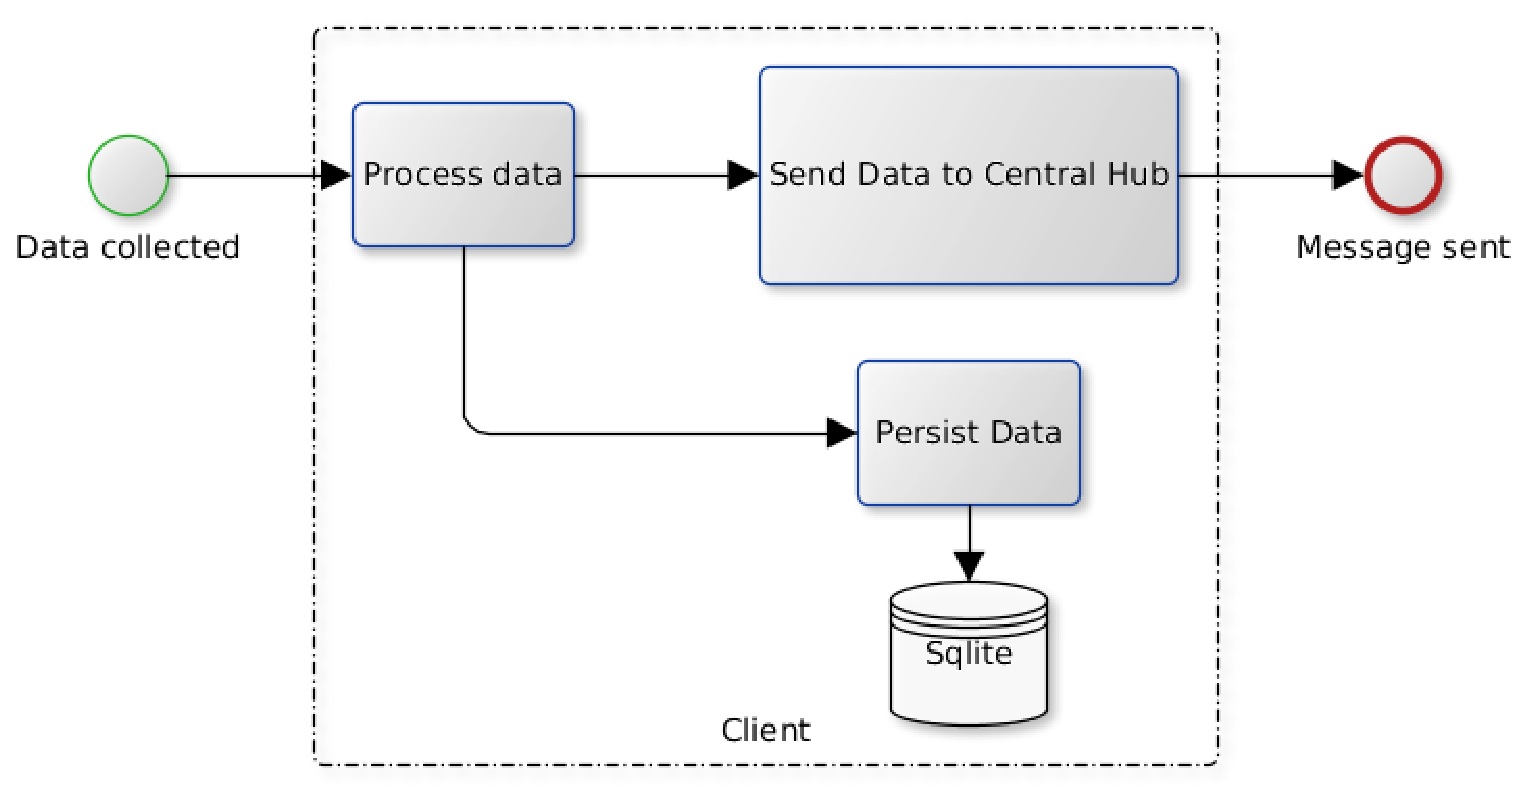
\includegraphics[width=2.5in]{client_diagram}
\caption{Sensor Node Diagram}
\label{sensor_diagram}
\end{figure}


\subsubsection{Central Hub}
The central hub must be able to process a high volume of messages coming from the sensor nodes and to answer requisitions for information from network users.

The central hub was implemented also using raspberry pi 2 model B running a computer program based on Tornado \cite{Tornado2015}, a RabbitMQ broker and  a web server based on the framework flask\cite{Flask}.

Tornado is a Python web framework and asynchronous networking library. By using non-blocking network I/O, Tornado can scale to tens of thousands of open connections, making it ideal for long polling, WebSockets, and other applications that require a long-lived connection to each user.\cite{Tornado2015}

The server is responsible for listening for messages posted on the RabbitMQ broker and collect the relevant data and persist them in its own SQLite  database. This database has information from all nodes composing the network.

The RabbitMQ broker is responsible for managing communications between nodes and the central hub.

The web server is an application with an REST API\cite{Fielding2000} responsible for providing users of the system with an method to visualize the data collected by the sensor network. It uses a lightweight server structure ideal for running in embedded systems.

The services implemented in the central hub may be divided between data collection and communication.

\begin{figure}[ht!]
\centering
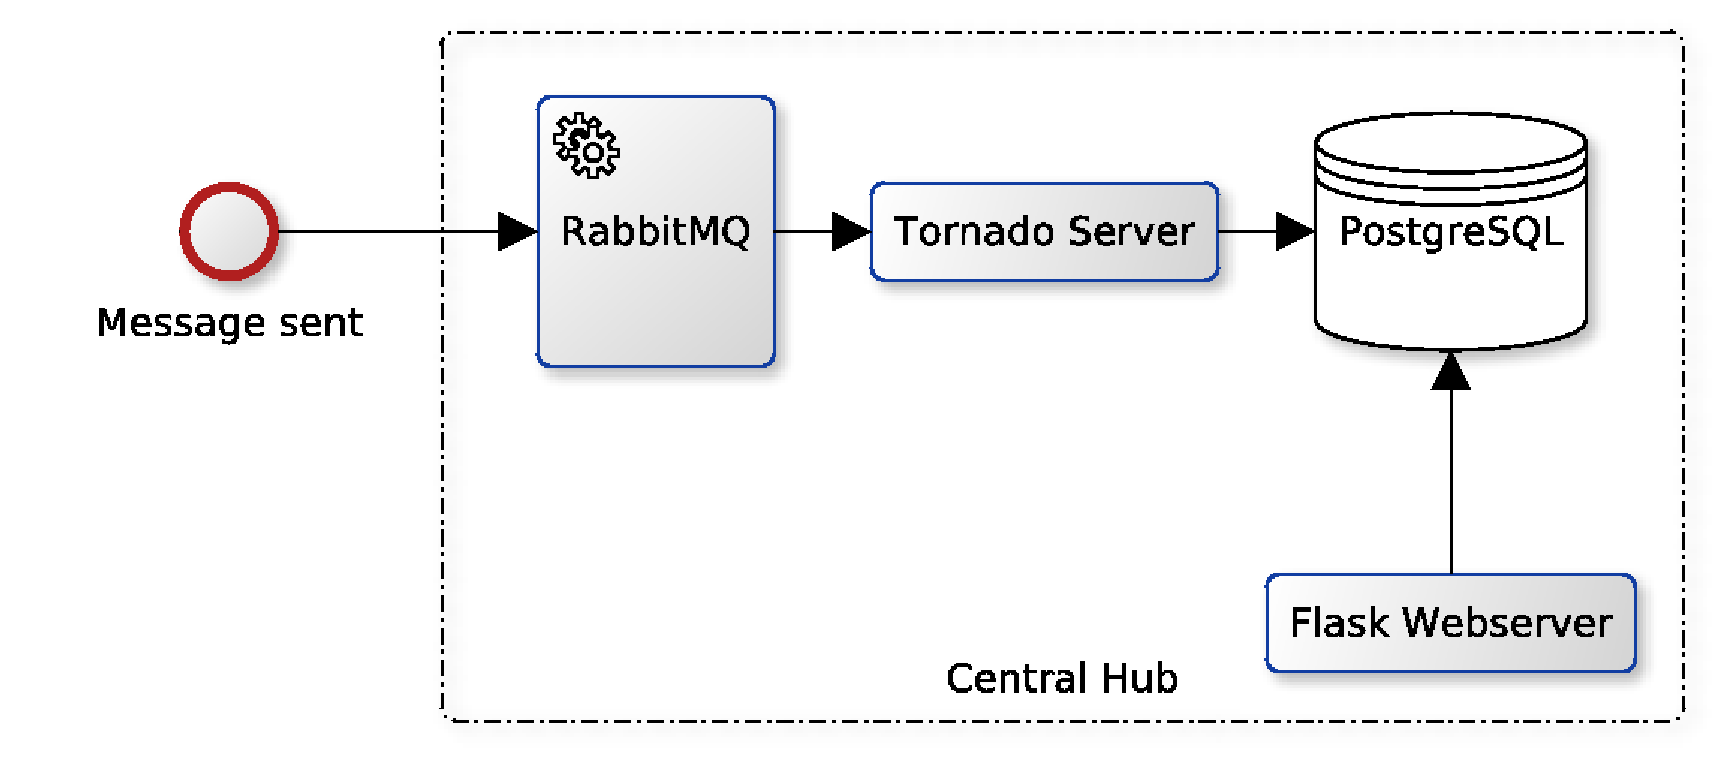
\includegraphics[width=2.5in]{system_diagram}
\caption{Central Hub Diagram}
\label{central_hub_diagram}
\end{figure}


\subsubsection{Message Protocol}
The messages are sent from the sensor node to the central  Hub using the MQTT protocol.

MQTT stands for MQ Telemetry Transport. It is a publish/subscribe, extremely simple and lightweight messaging protocol, designed for constrained devices and low-bandwidth, high-latency or unreliable networks. The design principles are to minimise network bandwidth and device resource requirements whilst also attempting to ensure reliability and some degree of assurance of delivery. These principles also turn out to make the protocol ideal of the emerging "machine-to-machine" (M2M) or "Internet of Things" world of connected devices, and for mobile applications where bandwidth and battery power are at a premium\cite{mqtt}.

MQTT is a publish/subscribe messaging system that allows clients to publish messages without concerning themselves about their eventual destination; messages are sent to an MQTT broker where they may be retained.

The messages' payloads are just a sequence of bytes, up to 256MB, with no requirements placed on the format of those payloads and with the MQTT protocol usually adding a fixed header of two bytes to most messages.
 
Other clients can subscribe to these messages and get updated by the broker when new messages arrive. To allow for the variety of possible situations where MQTT can be put to use, it lets clients and brokers set a "Quality of Service" on a per-message basis from "fire and forget" to "confirmed delivery". MQTT also has a very light API, with all of five protocol methods, making it easy to learn and recall, but there's also support for SSL-encrypted connections and username/password authentication for clients to brokers.

The broker utilized in the implementation was RabbitMQ through the python package Pika. Pika is a pure-Python implementation of the AMQP 0-9-1 protocol that tries to stay fairly independent of the underlying network support library\cite{Pika}.
The model takes into account the need for constant data analysis and transmission of high volumes of messages in a heavy electronic noise environments.
\subsubsection{Message Format}
The message payload is formatted using in the Json format.
JSON (JavaScript Object Notation) is a lightweight data-interchange format\cite{Json}.
Each information corresponds to a key-value par that can be read easily by both human and computer programs.
\begin{lstlisting}
{
    "timestamp": "2015-07-16 15:40:49.218438",
    "data": {
        "ilumination": 210,
        "noise": 123,
        "carbon_monoxide": 170,
        "temperature": 51,
        "humidity": 127
    },
    "id": 307
}

\end{lstlisting}
\subsection{Implementation and tests}
To validate the proposed system a prototype was implemented to collect temperature, humidity, levels of flammable gas and luminance data to monitor the work conditions of a computer data server room. To maintain the proper conditions of the machines in these environments the temperature and humidity must be maintained at low levels. In the other way the luminance levels need to meet the minimum levels required to not strain workers eyesight. As a safety measure the levels of flammable gases as butane, methane and propane were also monitored. The prototype was used to assure that all 4 factors were in a range satisfactory for workers and machines. As a result of this implementation a data sample of 19315 measurements was extracted that is described in table I. The samples comprehend the period from September, 3rd, 2015 at 17:25:37 to September, 04th, 2015 at 14:08:27.

No messages were lost during testing.
\begin{table}[!ht]
\renewcommand{\arraystretch}{1.3}
\caption{Data Server environment factors}
\label{table_data}
\centering
\begin{tabular}{c||c||c||c||c}
\hline
\bfseries Variable & Mean & STD & Min & Max \bfseries \\
\hline\hline
Temperature ($^{\circ}$C) & 27.097334 & 1.162900 & 25 & 31 \\
Humidity (\%) & 35.382760 & 4.395421 & 26 & 45 \\
Luminance (lux) & 202.594512 & 445.754322 & 0 & 2055 \\
Gas (ppm) & 94.932747 & 17.561130 & 43 & 495 \\
\end{tabular}
\end{table}

The python Package matplotlib\cite{Hunter:2007} was used to create the following graphics:

On figure 3 it is possible to observe that the temperature in the room remains with little fluctuation with changes of only 6 degrees Celsius.

On figure 4 the humidity is shown and it is of note that the levels suffer little fluctuation.

On figure 5 the luminance levels are shown with a scale of 10 times the actual value in Lux meaning that the lighting in the room remain with levels of 200 Lux approximately that is inside the recommended for indoor work.

The figure 6 shows that the gas presence data contains 2 spikes that represent a test of the sensor in the beginning of the data collection and other more pronounced at approximately 21:45 as a result of testing with different gas sources.

\begin{figure}[ht!]
\centering
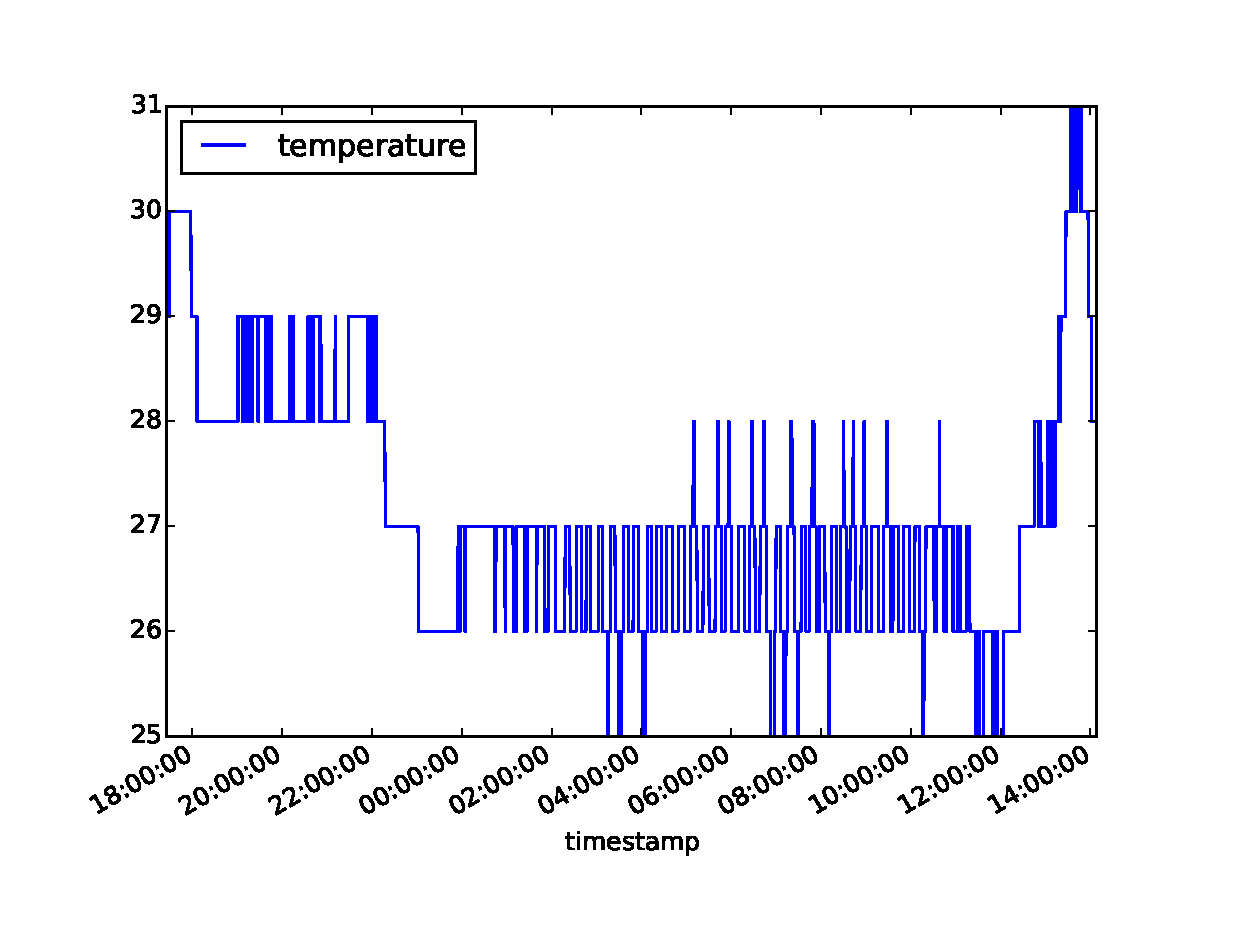
\includegraphics[width=3.5in]{plot_temperature}
\caption{Temperature}
\label{temp_plot}
\end{figure}

\begin{figure}[ht!]
\centering
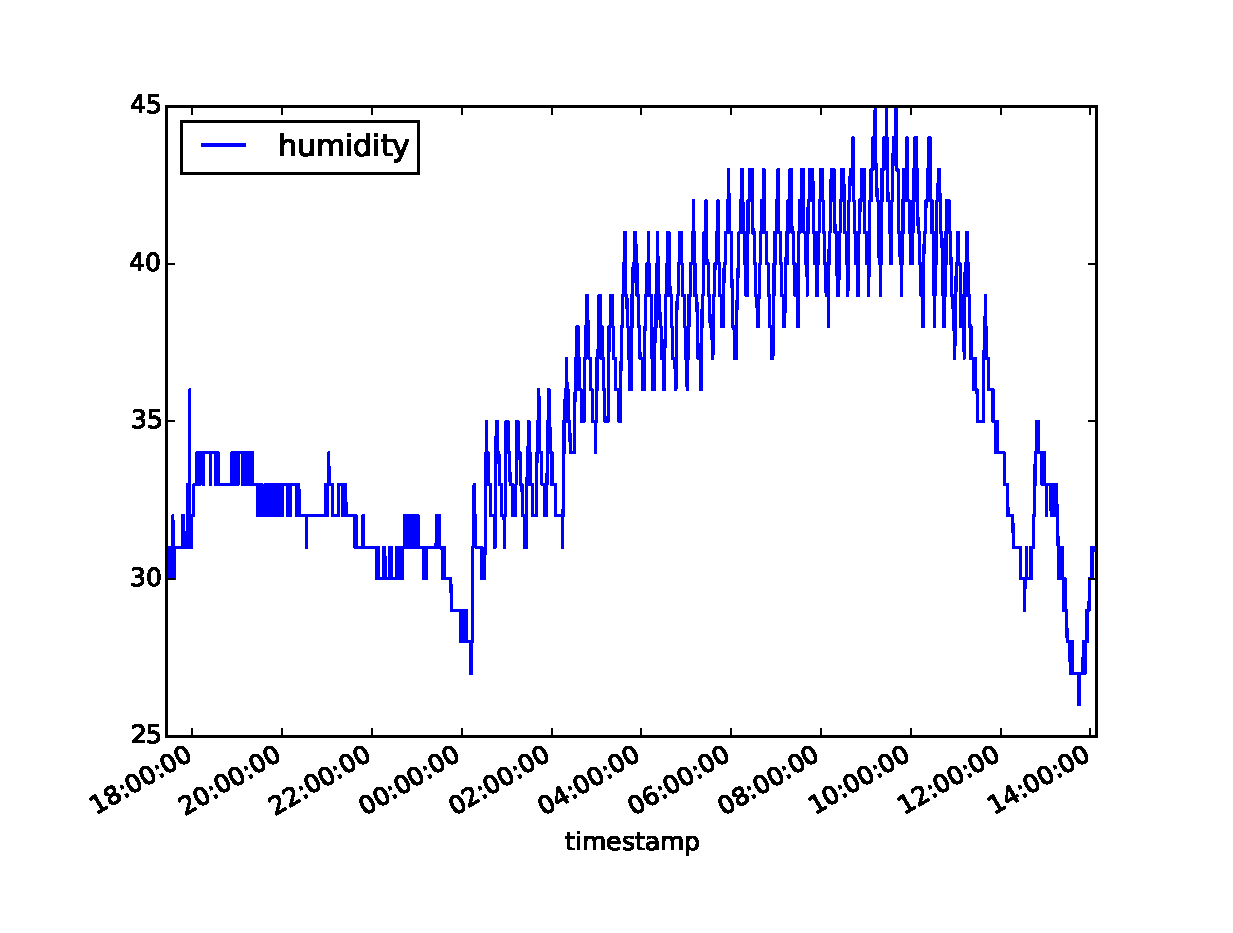
\includegraphics[width=3.5in]{plot_humidity}
\caption{Humidity}
\label{humidity_plot}
\end{figure}

\begin{figure}[ht!]
\centering
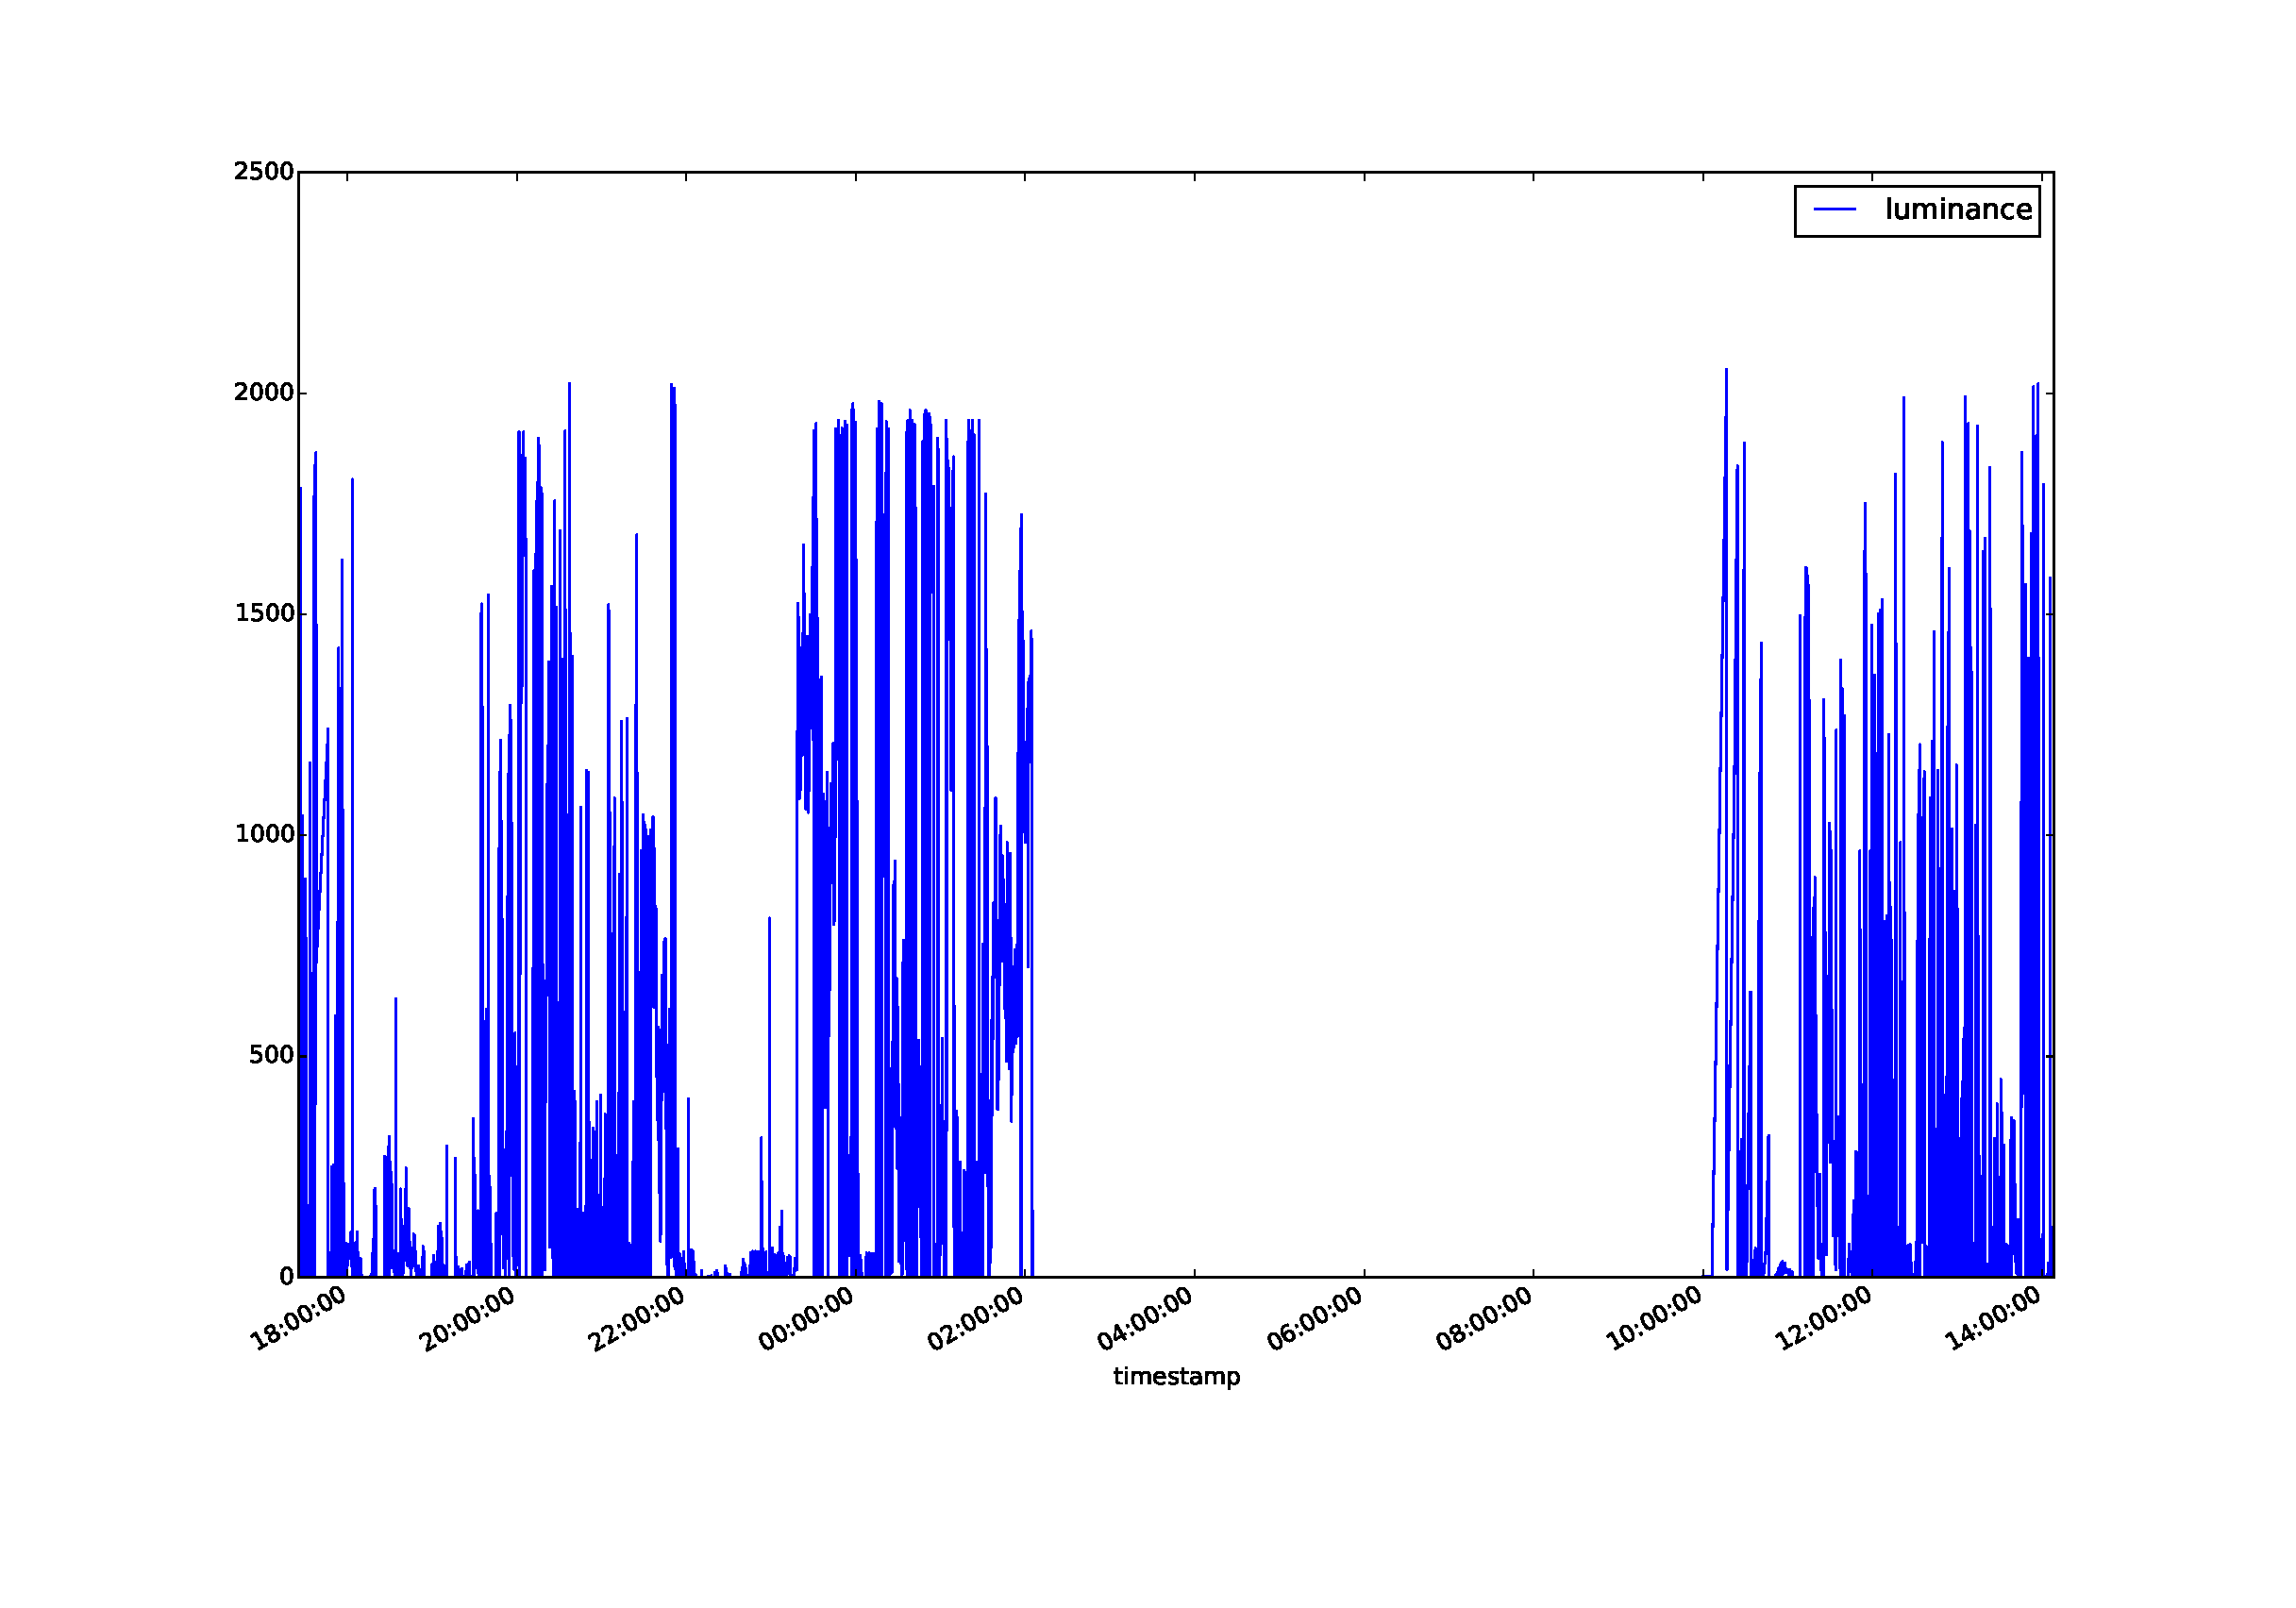
\includegraphics[width=3.5in]{plot_luminance}
\caption{Luminance}
\label{luminance_plot}
\end{figure}

\begin{figure}[ht!]
\centering
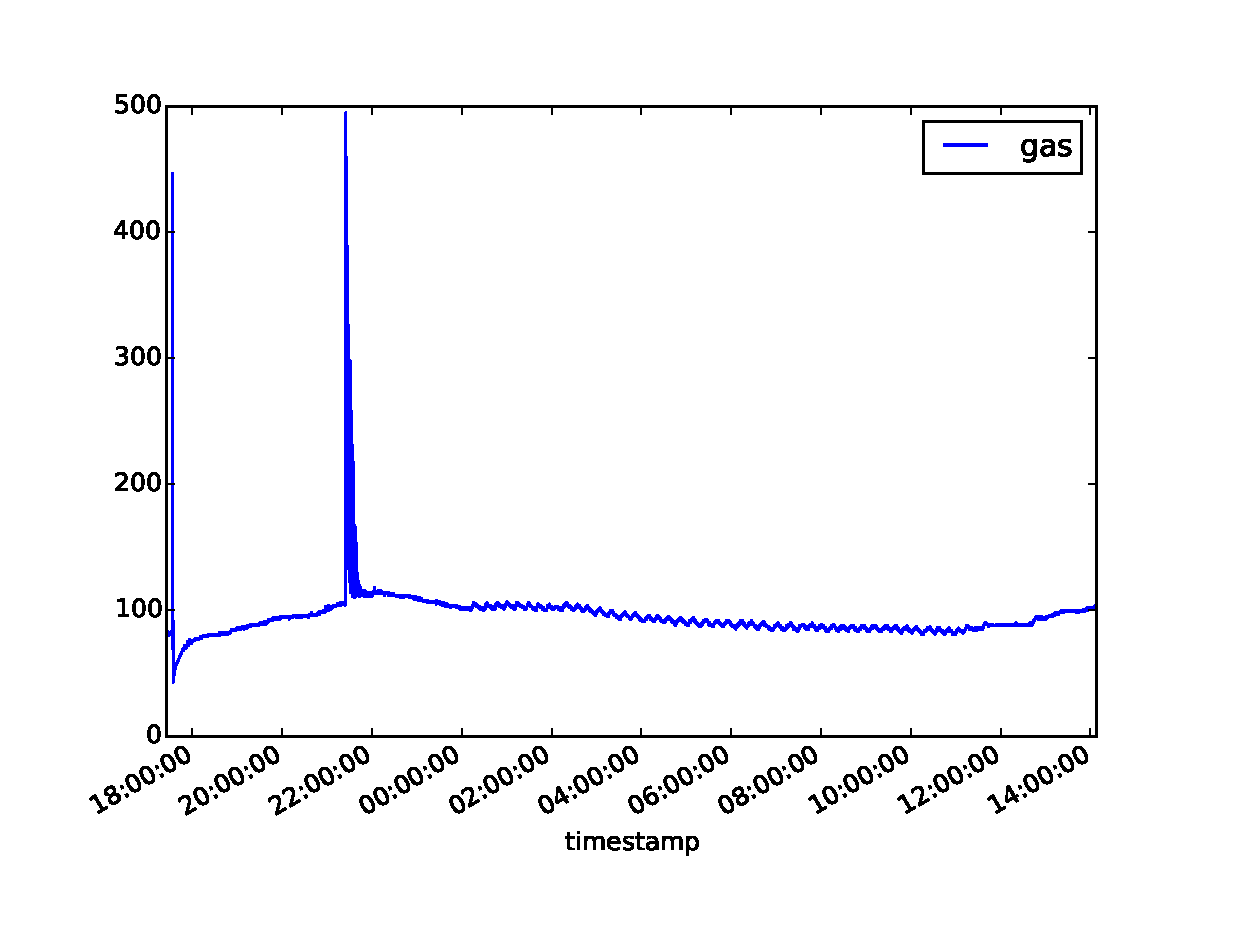
\includegraphics[width=3.5in]{plot_gas}
\caption{Gas presence}
\label{gas_plot}
\end{figure}

\subsection{Application of collected data}
According with Woo\cite{Woo2008} the workplace can make manifest latent mood disorders, destabilize, and aggravate symptoms and courses of mood disorders among workers. This is reinforced by Sarode\cite{Sarode2014} bad work conditions related to Noise, Lightning, air quality, temperature and humidity affected both the psychological and physiological welfare of the workers, causing such conditions as eye strain, fatigue, headache, back pain, and nausea.

The information collected by the WSN can be used to profile, make adjustments and improve work conditions in the monitored environment. These improvements may impact the productivity, quality and costs of workers.

The noise sensor information may be used to specify mufflers on combustion engines, the class of hear gear to be distributed to workers of a specific area or installation of acoustic insulation.

Luminance data may be used to adjust automatic levels of lighting.

Temperature and humidity data may be used to adjust Air conditioning systems.




\section{Conclusion}
In this article an Architecture for Wireless sensor networks for monitoring Environmental factors is presented.
Environmental monitoring through sensor networks is a promising technology. With the advances in the miniaturization of sensors and low power micro-controller systems these networks will become more prevalent and gain more applications. 
In the future other sensor nodes will be deployed in an office ambient to also monitor the luminance and noise. 

Others sensors may be used with this setup as hall sensors to monitor electrical energy consumption or flow rate sensors to monitor water consumption, river flow or sewers.

For long range monitoring further study will be necessary to choose the best network topology and technology with the best candidates being mesh networks over high frequency wireless. 

% use section* for acknowledgment
\section*{Acknowledgment}
The authors would like to thank their families for their love, care, kindness, patience, and unfailing trust.
%-------------------------------------------------------------------------
\bibliographystyle{ieeetr}
\bibliography{artigo_chilecon_108}

\end{document}

